% Created 2022-08-26 vie 13:56
% Intended LaTeX compiler: pdflatex
\documentclass[12pt]{article}
\usepackage[utf8]{inputenc}
\usepackage[T1]{fontenc}
\usepackage{graphicx}
\usepackage{grffile}
\usepackage{longtable}
\usepackage{wrapfig}
\usepackage{rotating}
\usepackage[normalem]{ulem}
\usepackage{amsmath}
\usepackage{textcomp}
\usepackage{amssymb}
\usepackage{capt-of}
\usepackage{hyperref}
\usepackage[spanish]{babel}
\usepackage{graphicx,geometry}
\geometry{ a4paper, left=1in, right=1in, top=1in, bottom=1in }
\renewcommand\familydefault{\sfdefault}
\usepackage{sectsty}
\sectionfont{\normalfont\large }
\usepackage{tabularx}
\usepackage{listings}
\lstdefinestyle{mystyle}{
numbers=left,
showspaces=false,
frame=leftline,
showspaces=false,
showstringspaces=false,
showtabs=false,
numberstyle=\tiny,
}
\lstset{
style=mystyle,
literate={á}{{\'a}}1
{é}{{\'e}}1
{í}{{\'{\i}}}1
{ó}{{\'o}}1
{ú}{{\'u}}1
{Á}{{\'A}}1
{É}{{\'E}}1
{Í}{{\'I}}1
{Ó}{{\'O}}1
{Ú}{{\'U}}1
{ü}{{\"u}}1
{Ü}{{\"U}}1
{ñ}{{\~n}}1
{Ñ}{{\~N}}1
{¿}{{?``}}1
{¡}{{!``}}1
}
\makeatletter
\usepackage{fancyhdr}
\pagestyle{fancy}
\usepackage{mdframed}
\BeforeBeginEnvironment{minted}{\begin{mdframed}}
\AfterEndEnvironment{minted}{\end{mdframed}}
\author{Luis Eduardo Galindo Amaya (1274895)}
\date{2022-08-25}
\title{Esquematización de los componentes de entorno de desarrollo integrado}
\hypersetup{
 pdfauthor={Luis Eduardo Galindo Amaya (1274895)},
 pdftitle={Esquematización de los componentes de entorno de desarrollo integrado},
 pdfkeywords={},
 pdfsubject={},
 pdfcreator={Emacs 26.3 (Org mode 9.1.9)}, 
 pdflang={Spanish}}
\begin{document}


\newcommand{\docente}{Manuel Castañón-Puga}
\newcommand{\asignatura}{Herramientas de Desarrollo de Software (40017)}
\newcommand{\semestre}{2022-2}

\newcommand{\miportada}[1]{
	\begin{titlepage}
		\vspace*{0.75in}
		\begin{flushleft}
			\sffamily
			\large #1       \\
			\Huge 
            \@title         \\
			\hrulefill
			\vspace{0.25in} \\
			\Large \@author \\
			\vspace*{\fill}
            
\includegraphics[width=\textwidth]{../includes/filler.png} \\
			\vspace*{\fill}
			\large
			\begin{tabular}{|l|l|}
              \hline
			  Asignatura & \asignatura \\
			  Docente    & \docente    \\
			  Fecha      & \@date      \\
              \hline
			\end{tabular}
		\end{flushleft}
	\end{titlepage}
}

\fancyhf{}
\lhead{ \asignatura }
\rhead{ \semestre }
\rfoot{Página \thepage}

\setlength\parindent{0pt}   % eliminar el intentado
\setlength{\parskip}{1.2em}
% \maketitle

\thispagestyle{empty}
\begin{center}
	{\large
		UNIVERSIDAD AUTÓNOMA DE BAJA CALIFORNIA \\
		Facultad de Ciencias Químicas e Ingeniería }
	\vspace{0.25in} \\
	Programa de Ingeniero en Software y Tecnologías Emergentes
\end{center}

\section*{Información De La Materia}
\label{sec:org184e77f}
\begin{mdframed}
\begin{description}
\item[{Asignatura}] \asignatura .
\item[{Grupo y Periodo}] 341 (2022-2) .
\item[{Docente}] \docente .
\end{description}
\end{mdframed}

\section*{Información De La Actividad}
\label{sec:orged7e074}
\begin{mdframed}
\begin{description}
\item[{Nombre de la actividad}] Esquematización de los componentes de entorno de desarrollo integrado
\item[{Fecha}] 2022-08-25
\item[{Lugar}] Edificio 6E, Salón 204.
\item[{Carácter de la actividad}] Individual.
\item[{Participante(es)}] Luis Eduardo Galindo Amaya (1274895).
\end{description}
\end{mdframed}

\section*{Mapa Mental}
\label{sec:org21f0c71}
\begin{center}
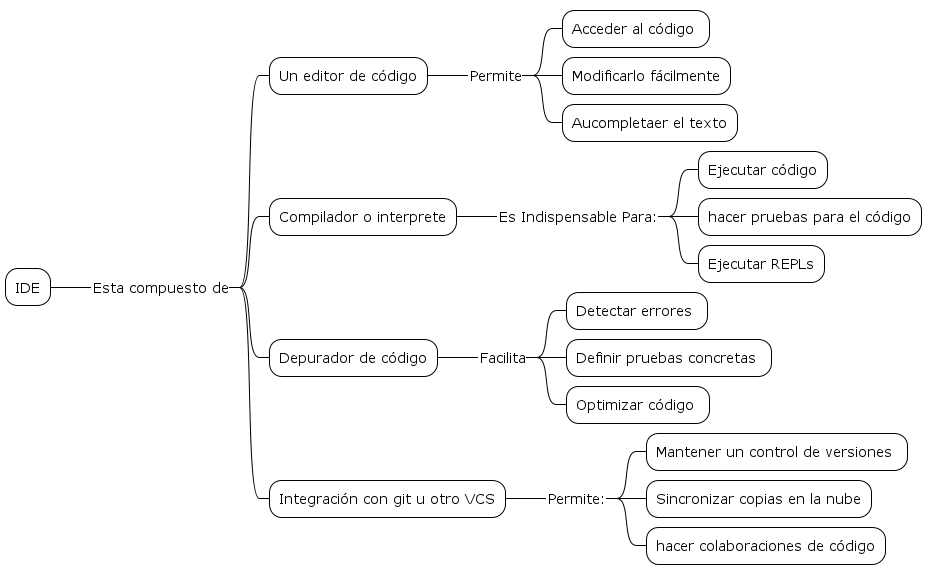
\includegraphics[width=13cm]{./img/mapa.png}
\end{center}

\section*{Reflexión}
\label{sec:org4bbdfc9}
\begin{mdframed}
Como profesionales en el diseño de software podemos es necesario que podamos operar herramientas como IDEs para poder integrarnos rápidamente en los equipos, obviamente integrarse en un nuevo grupo de trabajo es tardado pero si se conoce previamente la herramienta de trabajo la transición puede ser menos dolorosa y mas orientada a los asuntos meramente técnicos.
\end{mdframed}

\begin{center}
Doy fe de que toda la información dada es  completa y correcta. \\
\begin{center}

\includegraphics[width=3cm]{../includes/firma.png}
\end{center}
Luis Eduardo Galindo Amaya (1274895)
\end{center}
\end{document}
